\documentclass{standalone}
\usepackage{tikz}
\usetikzlibrary{shapes.geometric, arrows}
\tikzset{arrow/.style = {thick,->,>=stealth}}

\begin{document}
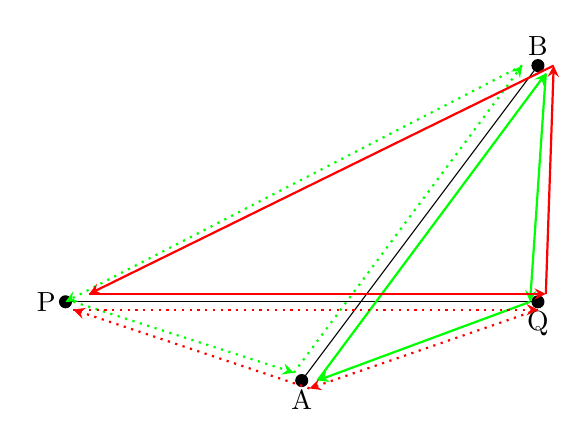
\begin{tikzpicture}

\draw (0,1) node[anchor=east] {P} -- (6,1) node[anchor=north] {Q};
\draw (3,0) node[anchor=north] {A} -- (6,4) node[anchor=south] {B};



\draw[fill=black] (0,1) circle (.5ex);
\draw[fill=black] (6,4) circle (.5ex);
\draw[fill=black] (3,0) circle (.5ex);
\draw[fill=black] (6,1) circle (.5ex);

\draw[arrow, dotted, green] (0.1, 1) -- (2.9, 0.1);
\draw[arrow, dotted, green] (2.9, 0.1) -- (5.8, 4);
\draw[arrow, dotted, green] (5.8, 4) -- (0, 1);

\draw[arrow, green] (3.2, 0) -- (6.1, 3.9);
\draw[arrow, green] (6.1, 3.9) -- (5.9, 1);
\draw[arrow, green] (5.9, 1) -- (3.2, 0);

\draw[arrow, red] (6.1, 1.1) -- (6.2, 4);
\draw[arrow, red] (6.2, 4) -- (0.3, 1.1);
\draw[arrow, red] (0.3, 1.1) -- (6.1, 1.1);

\draw[arrow, dotted, red] (0.1, 0.9) -- (6, 0.9);
\draw[arrow, dotted, red] (6, 0.9) -- (3.1, -0.1);
\draw[arrow, dotted, red] (3.1, -0.1) -- (0.1, 0.9);

\end{tikzpicture}
\end{document}